\documentclass[10pt,twoside]{article}
\usepackage[utf8]{inputenc}
\usepackage{amsmath}
\usepackage{amsfonts}
\usepackage{amssymb}
\usepackage[spanish,es-noshorthands]{babel}
\usepackage[T1]{fontenc}
\usepackage{lmodern}
\usepackage{graphicx,hyperref}
\usepackage{tikz,pgf}
\usepackage{multicol}
\usepackage[papersize={6.5in,8.5in},width=5.5in,height=7in]{geometry}
\usepackage{fancyhdr}
\pagestyle{fancy}
\fancyhead[LE]{
\includegraphics[height=12pt]{Images/logo-colegio.png} Álgebra $8^{\circ}$}
\fancyhead[RE]{}
\fancyhead[RO]{\textit{Germ\'an Avenda\~no Ram\'irez, Lic. U.D., M.Sc. U.N.}}
\fancyhead[LO]{}

\author{Germ\'an Avenda\~no Ram\'irez, Lic. U.D., M.Sc. U.N.}
\title{\begin{minipage}{.2\textwidth}

\includegraphics[height=1.75cm]{Images/logo-colegio.png}\end{minipage}
\begin{minipage}{.55\textwidth}
\begin{center}
Taller 06, Productos notables\\
Álgebra $8^{\circ}$
\end{center}
\end{minipage}\hfill
\begin{minipage}{.2\textwidth}

\includegraphics[height=1.75cm]{Images/logo-sed.png} 
\end{minipage}}
\date{}
\begin{document}
\maketitle
Nombre: \hrulefill Curso: \underline{\hspace*{44pt}} Fecha: \underline{\hspace*{2.5cm}}
\section*{Repaso}
En las pasadas clases hemos visto como hacer determinar el cuadrado de un binomio y como hacer una suma por una diferencia. Recordemos que:
\subsection*{Cuadrado de un binomio}
\[(a\pm b)^{2}=a^{1}\pm 2ab+b^{2}\]
\textbf{Ejemplo:}
\begin{align*}
(3x+2y)^{2}&=(3x)^{2}+2(3x)(2y)+(2y)^{2}\\
&=9x^{2}+12xy+4y^{2}
\end{align*}
\subsection*{Suma por diferencia}
\[(a+b)(a-b)=a^{2}-b^{2}\]
\textbf{Ejemplo:}
\begin{align*}
(3x+4y)(3x-4y)&=(3x)^{2}-(4y)^{2}\\
&=9x^{2}-16y^{2}
\end{align*}
\section*{Otros productos notables}
Continuando con nuestro aprendizaje acerca de los productos notables tenemos los siguientes:
\subsection*{Cubo de un binomio}
\subsubsection*{Cubo de una suma}
\[(a+b)^{3}=a^3+3a^2b+3ab^2+b^3\]
\paragraph*{Demostración}
\begin{align*}
(a+b)^{3}&=(a+b)^{2}(a+b)\\
&=(a^{2}+2ab+b^2)(a+b)\\
&=a^2(a+b)+2ab(a+b)+b^2(a+b)\\
&=a^3+a^2b+2a^2b+2ab^2+ab^2+b^3\\
&=a^3+3a^2b+3ab^2+b^3
\end{align*}
\subparagraph*{Ejemplo:} Resolver $(x+4)^3$

Usamos el producto notable anterior así:
\begin{align*}
(x+4)^3&=x^3+3(x)^2(4)+3(x)(4)^2+4^3\\
&=x^{3}+12x^2+48x+64
\end{align*}
\subsubsection*{Cubo de una diferencia}
\begin{align*}
(a-b)^3&=(a-b)^2(a-b)\\
&=(a^2-2ab+b^2)(a-b)\\
&=a^2(a-b)-2ab(a-b)+b^2(a-b)\\
&=a^3-a^2b-2a^2b+2ab^2+ab^2-b^3\\
&=a^3-3a^2b+3ab^2-b^3
\end{align*}
\paragraph*{Ejemplo:}

Resolver $(3x-2y)^3$

Procedemos así:
\begin{align*}
(3x-2y)^3&=(3x)^3-3(3x)^2(2y)+3(3x)(2y)^2-(2y)^3\\
&=3^3x^3-3(3^2x^2)(2y)+9x(2^2y^2)-2^3y^3\\
&=27x^3-3(9x^2)(2y)+9x(4y^2)-8y^3\\
&=27x^3-54x^2y+36xy^2-8y^3
\end{align*}
Por último debemos recordar que si olvidamos un producto notable o éste no aplica para el caso a resolver, entonces debemos usar la propiedad distributiva como en el siguiente ejemplo:
\begin{align*}
(2x-1)(x^2-4x+6)&=2x(x^2-4x+6)-1(x^2-4x+6)\\
&=2x^3-8x^2+12x-x^2+4x-6\\
&=2x^3-9x^2+16x-6
\end{align*}
\subsection*{Conexión con la geometr\'{i}a:}
Como se puede esperar, hay interpretaciones geométricas para muchos de los conceptos algebraicos. Tendremos la oportunidad de ver la conexión entre álgebra y geometría en la solución del siguiente problema.
\subsubsection*{Problema}
De un rectángulo de 16 pulgadas por 12 pulgadas se quita un cuadrado de lado $x$ en cada esquina del rectángulo para luego doblar las pestañas hacia arriba y construir así una caja como se muestra en la figura. Encuentre los polinomios que representan el volumen y la superficie exterior de la caja.
\begin{center}
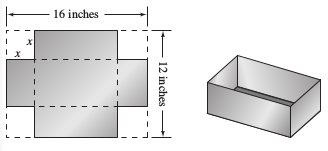
\includegraphics[scale=1]{Images/caja_12in.png} 
\end{center}
\paragraph*{Solución:}

El largo de la caja será $15-2x$, el ancho $12-2x$ y la altura $x$. Por tanto su volumen será ($V=largo\times ancho \times alto$):
\begin{align*}
(16-2x)(12-2x)x&=16(12x-2x^2)-2x(12x-2x^2)\\
&=192x-32x^2-24x^2+4x^3\\
&=4x^3-56x^2+192x
\end{align*}
Ésta última expresión $4x^3-56x^2+192x$ representa el volumen de la caja.

Ahora para calcular la superficie externa de la caja basta con restar al área del rectángulo original las cuatro esquinas que se cortaron. Luego el polinomio que representa la superficie externa de la caja es: 
$16(12)-4x^2=192-4x^2$
\end{document}
